%========================================================================================
% TU Dortmund, Informatik Lehrstuhl VII
%========================================================================================
\chapter{Kapitel 3 - Physik}
\label{Kapitel 4}

Um die Bewegungen des Ball möglichst realistisch und nachvollziehbar zu realisieren und somit dem Nutzer ein echtes Spielgefühl zu vermitteln, müssen einige physikalische Eigenschaften der "{}echten Welt"{} ins Spiel implementiert werden. In diesem Fall heißt es, dass die Reflexionen eines Balls auf einer Oberfläche richtig berechnet werden müssen. Dementsprechend müssen auch Kollisionsabfragen dafür realisiert werden. Des Weiteren soll die Bewegung des Balls innerhalb der Box korrekt berechnet werden sowie ein Gravitationsfaktor die Fallgeschwindigkeit beeinflussen können.

Da im Programm in jedem Durchlauf der Hauptschleife zuerst die Bewegungen und dann die Kollisionen bzw. die Reflexionen berechnet werden, wird auch in diesem Kapitel diese Reihenfolge beibehalten.
\section{Kapitel 3 - Bewegungen}
\label{Kapitel_4_-_Unterkapitel_1}
Die verschiedenen physikalische Eigenschaften des Balls werden in der Klasse BallPhysics verwaltet. Dazu gehören: Masse, Kraft, Gravitation und Geschwindigkeit.
%====================Kraft wird nicht benutzt!!================
%===================Wahrscheinlich noch ändern=================
Bei jedem Tick wird die Update-Methode des Balls aufgerufen, die wiederum für die Positionsbestimmung zunächst die Update-Methode der Klasse Ballphysics aufruft, die die aktuelle Geschwindigkeit berechnet. Da die Geschwindkeit als 3-dimensioneller Vektor gespeichert wird, ergibt sich daraus auch immer die Richtung in die der Ball sich bewegt. Dabei wird zunächst die Beschleunigung des Balls, die durch die Masse und die Gravitationskraft beeinflusst wird, berechnet und schließlich auf den Geschwindigkeitsvekor addiert.
 \begin{equation}
	    \label{beschleunigung}
	    Beschleunigung = (\frac{1}{Masse} + Gravitation) * t 
    \end{equation}
Mithilfe des Geschwindigkeitsvektor lässt sich dann die nächste Position des Balls bestimmen:
\begin{equation}
	    \label{beschleunigung}
	    Position_{neu} = Position_{alt} + Geschwindikeit_{neu} * t 
    \end{equation}
Schließlich werden dann basierend auf der neuen Position die Rendering-Informationen aktualisert (s. Kapitel --/--) 



\section{Kapitel 3 - Reflexion}
\label{Kapitel_4_-_Unterkapitel_2}

Nachdem die Positionen aktualisert wurden wird geprüft, ob an den neuen Positionen Kollisionen aufgetreten sind. Dies geschieht in der CollisionResolver-Klasse. Die Funktion resolveCollisions(Ball* ball, Rackets* rackets, Box* box) wird von der Hauptschleife aus aufgerufen und überprüft zuerst die Kollision des Balls mit der Box bzw. mit den 6 Ebenen der Box und dann die Kollision mit dem Schläger.
Die Ebenen wurden wie erwähnt in einer der Hesseschen Normalform ähnlichen Darstellung gespeichert, sodass der Abstand des Balls zu einer Ebene leicht berechnet werden kann.

\begin{figure}[h]
    \subfigure[]
          {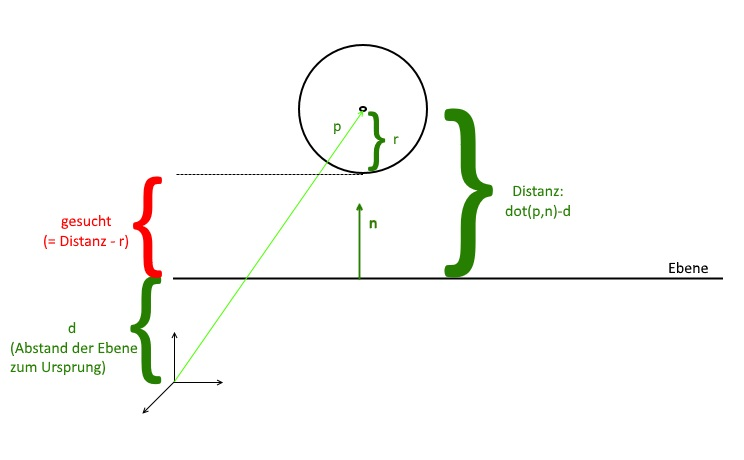
\includegraphics[scale=0.8]{bilder/collision}\label{fig_testbild_a}
    }
    \caption[Testbilder]{Übersicht der Kollisionsüberprüfung}
        \label{fig_testbild}
\end{figure} 

Da die Hessesche Normalform wie folgt aussieht,$ E: \vec x \cdot \vec n  = d $, und d der Abstand zum Ursprung ist, lässt sich die Formel umformen zu $ E: \vec x \cdot \vec n  - d = 0$. Diese Formel ist erfüllt wenn x auf der Ebene liegt. Ersetzt man also 0 durch eine Variable c, kann der Abstand von Punkt x zur Ebene genau ermittelt werden. In unserem Fall erlauben wir auch negative Abstände; negative Abstände entstehen dann durch Ballpositionen, die hinter der Ebene liegen (entgegen der Richtung des Normalvektors).
Der Abstand des Ballmittelpunkts zur Ebene ist also $c = \vec p\cdot \vec n - d $.

Damit der Ball aber bei zu hohen Gechwindigkeiten nicht hinter die Ebene gelangt und die Kollision nicht erkannt wird, wurde eine Kollisionsüberprüfung nach [hier Literatur einfügen] implementiert, die genau dies verhindern soll.